% This is a sample document using the University of Minnesota, Morris, Computer Science
% Senior Seminar modification of the ACM sig-alternate style. Much of this content is taken
% directly from the ACM sample document illustrating the use of the sig-alternate class. Certain
% parts that we never use have been removed to simplify the example, and a few additional
% components have been added.

% See https://github.com/UMM-CSci/Senior_seminar_templates for more info and to make
% suggestions and corrections.

\documentclass{sig-alternate}

\usepackage{color}
\usepackage[colorinlistoftodos]{todonotes}
\usepackage{graphicx}
\usepackage[ruled]{algorithm2e}
\usepackage{amssymb}

\definecolor{Teal}{RGB}{2,132,130}
\newcommand{\allcomments}[1]{{#1}}
\newcommand{\hfcomment}[1]{\textcolor{Teal}{\allcomments{Henry: {#1}}}}

%%%%% Uncomment the following line and comment out the previous one
%%%%% to remove all comments
%%%%% NOTE: comments still occupy a line even if invisible;
%%%%% Don't write them as a separate paragraph
%\newcommand{\mycomment}[1]{}

\begin{document}

% --- Author Metadata here ---
%%% REMEMBER TO CHANGE THE SEMESTER AND YEAR AS NEEDED
\conferenceinfo{UMM CSci Senior Seminar Conference, December 2015}{Morris, MN}

\title{Modern Approaches to the Rich Vehicle Routing Problem}

\numberofauthors{1}

\author{
% The command \alignauthor (no curly braces needed) should
% precede each author name, affiliation/snail-mail address and
% e-mail address. Additionally, tag each line of
% affiliation/address with \affaddr, and tag the
% e-mail address with \email
\alignauthor
Henry F. R. Fellows\\
	\affaddr{Division of Science and Mathematics}\\
	\affaddr{University of Minnesota, Morris}\\
	\affaddr{Morris, Minnesota, USA 56267}\\
	\email{fello056@morris.umn.edu}
}

\maketitle
\begin{abstract}

The Rich Vehicle Routing Problem is a class of problems that revolve around finding the most optimal route for a certain set of deliveries. Obtaining approximate solutions to these computationally hard problems is both economically valuable and \hfcomment{academically interesting?}. Despite a long history of research in the field, new methods and approaches to specific subproblems are frequently introduced. This paper summarizes the problem, its applications, recent algorithms and approaches.


\end{abstract}

\keywords{Vehicle Routing Problem, Black-box optimization, Genetic Algorithms, Probability Collectives, Distributed Systems, \hfcomment{Reviewers! skip to the end to read notes!}

\section{Introduction}
\label{sec:intro}
Routing is a deeply pervasive feature of the modern world. From the point-to-point navigation of everyday driving to the shipping of bulk freight, the task of creating those routes has been increasingly automated. The long term trend towards self-driving vehicles means that computers will soon control the entire process of transportation; aside from selecting a departure and destination, humans need no longer be involved. Software to create routes for school buses, mail deliveries and garbage trucks have been in use for decades; everything from Amazon to Uber uses these systems on a daily basis. The problem of finding efficient routes quickly is still an ongoing problem in the real world. The exact impact of improvements in routing is difficult to measure, but in 2011, the external costs of traffic jams in the EU were 1-2\% of GDP\cite{Caceres-Cruz:2014}. \hfcomment{ANOTHER NUMBER http://www.rita.dot.gov/bts/sites/rita.dot.gov.bts/files/publications/freight_shipments_in_america/html/entire.html} A small improvement - say five percent - in routing efficiency represents a staggering amount of money. The general case of routing is the traveling salesman problem. The traveling salesman problem asks for the shortest route which passes through each point once. Assuming that each pair of points is connected by a link, the number of potential routes is $\tfrac{1}{2}n!$, which grows extremely quickly, and is significant even for small values. For $n=10$, the number of routes reaches $1814400$. The traveling salesman problem is in a class of problems known as NP-complete. Although it has not yet been proven, it is considered likely that there is no algorithm for NP-complete problems that allows them to be solved quickly. Fortunately, solutions of NP-complete problems are easy to verify. In practice, the traveling salesman problem is too abstract for real-world routing problems, and so a variant was proposed that better represents the challenges of routing vehicles.

\subsection{Routing in the real world}
\label{ssec:real}
Routing in the real world is often a complicated and messy affair. The vehicle has to have enough capacity for all of its deliveries, and often, customers expect that the vehicle arrives near a specified time. New stops may be added during the day, or the exact demand of each customer might not be known ahead of time. In some cases, the customer might not know how much of a product they need until the vehicle arrives. Dealing with these types of problems is the domain of the Rich Vehicle Routing Problem.
\section{The Vehicle Routing Problem}
\label{sec:VRP}

\begin{figure}
\centering
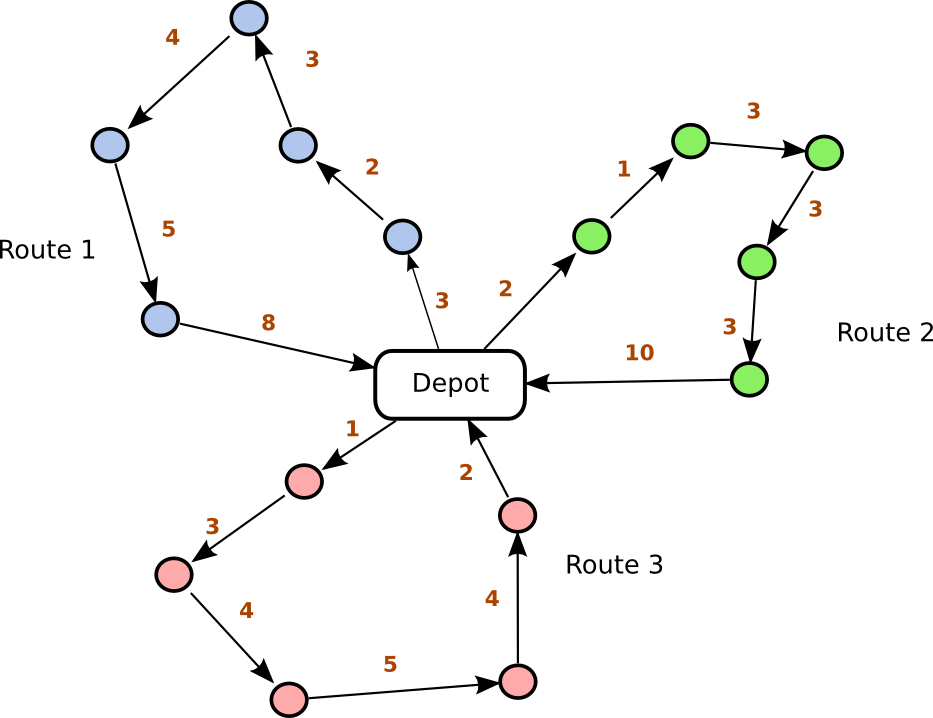
\includegraphics[width=3in, keepaspectratio]{vrp1.png}
\caption{Example of the VRP}
\hfcomment{Needs to replaced w/own image.}
\label{fig:VRPgraph}
\end{figure}

Originally titled the Truck Dispatching Problem, the original formulation of the Vehicle Routing Problem (VRP) was created by G. B. Danzig and J. H. Ramser in 1959\cite{Danzig:1959}. The premise of the problem is that each vehicle (or truck), has a limited capacity and the fleet must make deliveries to as many customers as possible, starting from a specific location known as a depot\cite{Caceres-Cruz:2014}. Alternatively, the vehicles may have to make multiple deliveries in order to satisfy all of the customers. A measure that is also considered worth minimizing is the maximum tour length - the longest single route taken by one truck. Danzig and Ramser note that if the total capacity of a vehicle is greater than the total demand of the customers, the problem is mathematically identical to the traveling salesman problem, because the . There has been a great deal of research done on the original VRP, and recent research focuses on versions of the VRP with different constraints or multiple constraints simultaneously. These variations of the Vehicle Routing Problem are collectively referred to as the Rich Vehicle Routing Problem\cite{Caceres-Cruz:2014} (RVRP).  In the following sections of, we discuss prominent variants of the RVRP.
\subsection{Decentralized Vehicle Routing Problem}
A common problem in rich vehicle routing literature is decentralized control, where each vehicle or depot is modeled as having an independent agent who makes decisions out of self-interest. However, pure self-interest can cause decisions that degrade the solutions of others. Imagine a vehicle which finds a route that fulfills a large number of deliveries extremely quickly; other vehicles might find that their routes force them to cross through this area where they cannot make any deliveries along the way. While it is highly efficient for the first vehicle, it is less efficient for all other vehicles. The ideal is to pursue optimal routes - both on the local (individual) scale, and on a global scale. Finding good methods of making decisions that allow for both autonomy and global utility is an ongoing research question. 
\subsection{Vehicle Routing Problem with Time Windows}
Another variant of the VRP is the vehicle routing problem with time window (VRPTW). The VRPTW describes the situation where the customer expects that the deliveries take place within a certain time interval. Unlike the estimates provided by shipping services, these constraints are set by the customers. A simple example is the constraint that deliveries are only accepted during business hours. This adds the dimension of time to the problem - the time it takes the truck to traverse nodes and to complete the delivery must be considered. The VRPTW is one of the more popular subproblems because deliveries without implicit or explicit time constraints are rare. In practice, the time window constraint is rarely found without other constraints; industrial settings tend to consider the VRPTW to be the base problem for real-world settings. 
\subsection{Approaches}
In general the approaches used to solve the VRP are approximate methods; they intend to find 'good', not perfect solutions. The algorithms tend to use simple rules to guess solutions, and the process of narrowing down or perfecting these guesses is known as optimization. \hfcomment{History, maybe?}. Most modern methods of solving the VRP belong to the blackbox style of optimization; blackbox optimization is used when a problem does not have a formal algebraic model, or the model is too computationally expensive \cite{Amaran:2014}. The VRP does have a very good model, but it is extremely computationally expensive to use it, and so the natural choice is to use blackbox methods. The common feature of blackbox methods is the use of stochastic (random) elements, especially in selecting starting states. This makes blackbox methods into a double edged sword; they are often effective at solving otherwise intractable problems, but the solutions frequently fail to produce any insight into the problem. Stochastic decision making makes it hard to determine why the algorithm provides a specific solution. 

\hfcomment{Maybe: The preference for blackbox methods may be a reflection of the difficulty in finding/improving [non-guessing] algorithms (or, perhaps equivalently, of the inherent computational limitations of calculating a perfect answer to the VRP)}

\section{Genetic and Memetic Algorithms}
A genetic algorithm (GA) is a type of problem-solving that is inspired by natural selection. It is often used to find solutions for processes that are not well understood, but can be modeled well. In the case of the VRP, the problem is both known and modeled well, but the approximate solution given by a well-made genetic is often nearly as good, and much faster than computing the exact solution. 
The fundamental notion of a genetic algorithm is a \textit{genetic representation}, which is a means of representing an individual. By analogy, the representation is the genome of the individual.  A common representation is a fixed-length array of bits, but other representations are possible. These genetic representations are manipulated by genetic operators that simulate various processes. A mutation operator provides the analogue to biological mutation by altering values in the genetic representation; the traditional example is a function that flips bits based on a random number generator. The crossover operator represents reproduction - it combines traits from two (usually) individuals to produce a new individual. 
Genetic algorithms aim to improve their solutions, and they measure how 'good' a solution is by using a fitness function. Fitness functions are problem specific; in VRP, they measure if the individual solves the problem, and how good that solution is.

\begin{algorithm}
Initialize population\;
\While{not final state}{
	Select best individuals via fitness function\;
	Generate new individuals using genetic operators\;
	\ForEach{new individual}{
		\If{better than worst individual}{
		Replace that individual\;
			}
		}
	}
\Return best solution\;
\caption{Genetic Algorithm Pseudocode\label{GA}}
\end{algorithm}

The general form of a GA begins with initializing the population. The canonical example is creating individuals with random representations. Next, the algorithm enters its main loop; the loop is usually terminated when an iteration limit is reached, but other conditions are sometimes used that are specific to the problem. In the loop, the individuals are scored using the fitness function and the best are set aside for the next stage. The crossover operator is then applied to this group, and the mutation operator on the resulting individuals. Then, it evaluates each individual and replaces the worst members of the population with the new individuals. This process is repeated until the termination condition is reached.

\subsection{Human Assisted Routing}
\label{sec:humans}
\hfcomment{Not sure if it belongs here or in own section. Uses a GA as base algorithm.}

\begin{figure}
\centering
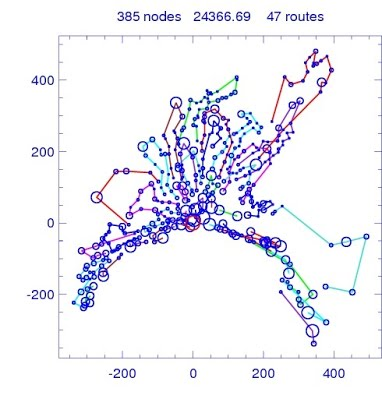
\includegraphics[width=3in, keepaspectratio]{vrp2.jpg}
\caption{To be example of selecting good/bad regions}
\hfcomment{Needs to replaced w/own image.}
\label{fig:Humangraph}
\end{figure}

Humans tend to be very good at solving visual problems, and this extends to the routing if the problem is displayed appropriately. We have a talent for deciding whether a given route is good or bad by simply looking at a diagram. Amazon's mechanical turk and similar platforms were created to allow developers to make use of human intelligence in solving computationally complex problems. Pursuing the approach of using humans to do things humans are good at anyways, S. Ismail, F. Legras and G. Coppin\cite{Ismail:2012} created a genetic algorithm that uses humans to determine how good a particular solution is. 


\begin{algorithm}
Initialize population\;
\While{number of interactions without improvement $< lt_{NI}$, and time $< T_{max}$}{
	Coherent algorithm goes here!\;
	Genetic algorithm stuff!\;
	Human selection suff!\;
	If good tags \;
	- higher selection probability\;
	- mutation operator not allowed\;
	If bad tags\;
	- lower selection probability\;
	- mutation operator encouraged\;
	Standard heuristic function\;
	Crossover\;
	}
\Return best feasible solution\;
\caption{Human Assisted Genetic Algorithm\label{HUMGA}}
\end{algorithm}
\hfcomment{describe in words, reference image}
\subsection{Hybrid Genetic Search with Advanced Diversity Control}
Adding time window constraints to customer demand and depot availability poses a significant challenge, especially in relation to the smaller proportion of solutions and the increased computational complexity caused by the increased search space. The opposing demands of temporal and spatial constraints is a particularly frustrating problem in the VRPTW.

The Hybrid Genetic Search with Advanced Diversity Control (HGSADC) address some of these challenges in the VRPTW, especially in route-duration constraints. The primary feature of the HGSADC is the different approach to diversity management in it's population. HGSADC adds diversity to its objectives as a term to be optimized, which allows it to avoid dead-end solutions. The algorithm is considered the current state of the art in the multi-depot vehicle routing problem with time windows\cite{Vidal:2013}.

\subsubsection{Algorithm and mechanics}
HGSADC is a complex algorithm, and cannot be fully described in this paper. What follows is a summary of the algorithm and the most notable features.


\begin{algorithm}
Initialize populations at $4\mu$ size\;
\While{number of interactions without improvement $< lt_{NI}$, and time $< T_{max}$}{
	Select parent solutions $P_1$ and $P_2$\;
	Create child $C$ from $P_1$ and $P_2$ (crossover)\;
	Educate $C$ (local search procedure)\;
	\If{$C$ infeasible}{
		Insert $C$ into infeasible subpopulation\;
		Repair with probability $P_{rep}$\;
	}
	\If{$C$ feasible}{
		Insert $C$ into feasible subpopulation\;
	}
	\If{maximum subpopulation size, $\mu$, reached}{
		Select survivors\;
	}
	\If{best solution not improved for $It_{div}$ iterations}{
		Diversify population\;
	}
		Adjust penalty parameters for infeasibility\;
	\If{number of iterations $modulo It_{dec} = 0$}{
		\hfcomment{aka every n iterations}\;
		Decompose the master problem\;
		Use HGSADC on each subproblem\;
		Reconstitute three solutions, and insert them in the
		population\;
	}
}
\caption{Hybrid Genetic Search with Advanced Diversity Control\label{HGSADC}}
\Return best feasible solution\;
\end{algorithm}
\hfcomment{This algorithm is actually frighteningly complex. It goes on for five pages, and it doesn't go into great detail, either. Also, the pseudocode should be above this}
HGSDAC evolves infeasible and feasible solutions as two separate subpopulations. Normally, infeasible ( `bad' ) solutions are removed from the population, but in the HGSADC, they are kept in a seperate subpopulation. The rationale is that this allows the algorithm to create a reserve of genetic diversity that can be used to get the population out of dead ends. Two random individuals are pulled from the combined population and the best of them is chosen to be a parent. The crossover operator is an applied to two parents, and the resulting child is educated.
 The education process is a limited local search that seeks to improve the child; if the child is still infeasible after this procedure, the repair procedure may be called. $P_{rep}$ is the probability that the repair operator is called; repair is a very intensive local search. Finally, the child is placed into an appropriate subpopulation. If a subpopulation exceeds a maximum size, a survivor selection stage is triggered. A number of individuals is removed until the population returns to the nominal population size $\mu$. The individual that is most similar in terms of fitness score and route to another individual is called the clone. Survivor selection iteratively removes the clone until the population size is returned to $\mu$. The purpose of this style of population management is to maintain diversity. A diversification round may be started if there has been $It_{div}$ iterations without improvement. \hfcomment{More when I understand it.} 
\subsubsection{Results} 
 It's crazy good. \hfcomment{More to come, but to say that it blows everything else out of the water is an understatement.}
\section{Agent-based models}
Agents are simply small decision making elements that typically have some internal state and the ability to make decisions based on this internal state. In optimization, a typical goal is for an agent to attempt to achieve some sort of optimal state. Agents (should) take actions to improve their state, and we describe this as the agent acting in its own interest. The function that returns the quantification of this local optimization is termed the local utility function, in contrast to the global, or system utility function. The global utility function describes how optimal the system is, which can be quite different from the local utility. 
\hfcomment{Make up definition? Agents are very poorly defined in literature.}
We have chosen to discuss two major approaches in modeling individuals for the decentralized VRP. The first is agent-based models, the more traditional approach, and the second is probability collectives, a relatively recent approach that has a legacy in genetic algorithms.

\subsection{Distributed reverse Vickrey auctions}

Saleh et al.\cite{Saleh:2012} were examining a version of the DCVRP where each depot and customer are treated as agents. The authors were interested in designing a system that encouraged near-optimal solutions while still being completely self-interested. They pursued this by building mechanisms that encouraged depots to offer an accurate estimate of minimum costs while still allowing the cost functions of each depot to remain private. \hfcomment{neat reverse vickrey auction info goes here once I understand game theory.}

\hfcomment{Maybe add very short pseudocode.}

The core feature of the algorithm is a reverse vickrey auction. Each depot $k$ submits a bid to each unassigned customer $j$ where $q_k^i \geq d_z$. Bids consist of the estimated costs of servicing the customer. The customer chooses the lowest bid satisfying their demands and notifies $k^*$. The depot $k^*$ may receive responses from other customers. From the given responses, the depot chooses the customer $j^*$ with the lowest insertion cost (the customer whose addition to  the vehicle's route will cause the least change  in the routing cost). Once the customer is assigned to a depot, the customer $j^*$ submits payment to depot $k^*$. The payment is equal to the second lowest offer of the game. This, combined with the fact that bids are sealed, encourages depots to provide the lowest possible rate (because if they win, they are still paid more than the estimate). The completion of these steps is a single auction round, and many rounds may take place until every customer is assigned. Once the auction rounds are complete, the depot can apply other optimization strategies to its routes, or in the case of small routes, an exact solution.

\subsection{Probability Collectives}
\label{ssec:PC}
Probability Collectives (PC) takes a different approach to selecting a good solution. Instead of attempting to evolve an exemplary individual in a population in the method of genetic or memetic algorithms, probability collectives selects optimal strategy for each agent\cite{Kulkarni:2008}. A PC agent is a self-interested, learning individual that selects a strategy with the highest probability of optimizing the local and global objectives. In contrast to the Distributed Reverse Vickrey Auction, the agents willingly and freely share information about their strategies, and the cost function is global.

\subsubsection{Mechanics of Probability Collectives}
The general form of PC in the context of VRP is as follows, along with the flowchart below. Imagine you have $N$ agents, which can be depots or trucks, each having a set $X$ of strategies, of (potentially variable) length $m$. The strategies are most often routes in RVRP applications\cite{Vasirani:2008}, but can sometime be as large as entire sets of routes or as small as individual actions. The set is represented as $X_i=\{X_i^{[1]}, X_i^{[2]}, ..., X_i^{[m]}\}$. 

A strategy for agent $i$ is denoted as $X_i^{[r]}$, where $r$ is an identifier for that strategy. For each agent, assign a uniform probability, $1/m_i$ to all actions; the resulting probability of that strategy is signified by $q(X_i^{[r]})$. The agents then selects a random action $r$ and a sampling of random actions from other agents. The resulting set, the `combined strategy set', $Y_i^{[r]}=\{X_1^{[?]}, ...,X_i^{[r]}, ...,X_N^{[?]}\}$, represents a guess as to a potential future. Accordingly, for each of the strategy sets $Y_i^{[r]}$, compute the expected local utility - the measure of how good the solution is expected to be for the agent - using the following measure:
	\begin{equation}
	\textit{Exp. Utility of Agent } i^r =q_i^r\prod_{(i)}{q(x_{(i)}^{[?]})\cdot G(Y_i^{[r]})}
	\end{equation}
Where $q_i^r$ represents the probability of action $r$ for vehicle $i$, $(i)$ is the set of all agents excluding $i$, and $G$ is the function that computes global utility for a given set of strategies. $G$ is problem specific, but in the RVRP it could be a measure of unused capacity, unvisited destinations, maximum tour length or various combinations of measurements.

After computing the local utility, the next step is to update the probability of each action for all agents as follows:
	\begin{equation}
	q(X_i^{[r]})<-q(X_i^{[r]})-\alpha_{Step}\cdot q(X_i^{[r]})\cdot k_r^{update}
	\end{equation}
	
where $k$ \hfcomment{fixme} is the iteration, $\alpha_{step}$ is a constant that controls the amount of change each step. Typical values range are around $0.98$. 
	\begin{equation}
	k_r^{update} = \dfrac{\textit{Contrib. of Agent }i}{T_k}+S_i(q)+ln(q(X_i^{[r]}))
	\end{equation}
	
Here, temperature $T_k$ is a scalar that represents the relative importance of the of the contribution of agent $i$ over time. It is computed as $T_k=T_0/ln(k)$, and $T_0$ is the initial temperature. A example value might be $30$.
\hfcomment{So, the PC papers reference an $\alpha_{T}$, which might be jammed in the numerator to add a rate control. Might just skip.}
The contribution of Agent $i$ is then:
	\begin{equation}
	\textit{Contrib. Agent }i = \textit{Exp. Utility Agent }i^r - \textit{Exp. Global Utility}
	\end{equation}
	
The $S_i(q)$ term is the entropy of the combined strategy set. In information theory, Entropy is the average value of the information in a message. Probability collectives treats the combined strategy set as a message in order to find the set with the highest Entropy. As it increases, the probability distribution more clearly distinguishes the contribution of each strategy toward optimizing the expected global utility. When it reaches a maximum, it represents the set that has the most information about the probabilities of each strategy. Entropy is computed by:
	\begin{equation}
	S_i(q)=-\sum_{r=1}^{m_i}q(X_i^{[r]})\cdot ln(q(X_i^{[r]})
	\end{equation}
	
Which is the sum of every strategy $q(X_i^{[r]})$ times the natural logarithm of itself. Here, the algorithm checks to see if it will continue updating the global utility or it will terminate. If the probabilities of the combined strategy set have not changed by a constant amount, $\sigma$, or if the number of iterations ($k$) have reached a maximum, the strategies with the highest probabilities will be returned. Otherwise, the algorithm will continue updating the combined strategy set.

To summarize, if a strategy $r$ creates a larger contribution to the optimization of the objective than other strategies, the probability associated with $r$ increases by a larger amount. This entire process is repeated until the probability distribution converges or the maximum number of iterations are completed. 

\begin{figure}
\centering
\includegraphics[width=2in, keepaspectratio]{"Probability Collectives Diagram".pdf}
\caption{Probability Collectives Algorithm.}
\label{fig:PCDiagram}
\end{figure}


\section{Conclusion}
\label{conclusion}
The vehicle routing problem is an important problem in real world logistics, and as in the field of optimization. The most performant algorithm in RVRP is hybrid genetic search with advanced diversity control, which is dominant within the scope of VRPTW. In decentralized RVRP variants, the specific constraints of each problem limit the comparability of each algorithm. The distributed reverse vickrey algorithm is within several percent of the best known solutions. Probability collectives is not as good in a straightforward sense, but it handles noisy and imperfect agent behaviors better than other distributed systems. 
Adding human intuition to optimization systems may be the next major step in improving routing systems. \hfcomment{(...)}
\section{Acknowledgements}
I'd like to thank caffeine, water, and stress; the raw elements that formed this paper. Harris L. Mayer's 1964 paper, ``Opacity Calculations, Past and Future" was a wonderful source of thematic inspiration.
\bibliographystyle{abbrv}
\bibliography{annotated_bibliography}  

% You must have a proper ".bib" file
%  and remember to run:
% latex bibtex latex latex
% to resolve all references

\hfcomment{So, clearly this is clearly very short: Earlier text blocking lead to a mistaken conclusion that the paper would be hitting 6 pages quickly. It also proved easier than expected to summarize some of the methods than expected. Nic McPhee says I should add more on results and I agree.}

\end{document}
